%%%%%%%%%%%%%%%%%%%%%%%%%%%%%%%%%%%%%%%%%
% University Assignment Title Page 
% LaTeX Template
% Version 1.0 (27/12/12)
%
% This template has been downloaded from:
% http://www.LaTeXTemplates.com
%
% Original author:
% WikiBooks (http://en.wikibooks.org/wiki/LaTeX/Title_Creation)
%
% License:
% CC BY-NC-SA 3.0 (http://creativecommons.org/licenses/by-nc-sa/3.0/)
% 
% Instructions for using this template:
% This title page is capable of being compiled as is. This is not useful for 
% including it in another document. To do this, you have two options: 
%
% 1) Copy/paste everything between \begin{document} and \end{document} 
% starting at \begin{titlepage} and paste this into another LaTeX file where you 
% want your title page.
% OR
% 2) Remove everything outside the \begin{titlepage} and \end{titlepage} and 
% move this file to the same directory as the LaTeX file you wish to add it to. 
% Then add \input{./title_page_1.tex} to your LaTeX file where you want your
% title page.
%
%%%%%%%%%%%%%%%%%%%%%%%%%%%%%%%%%%%%%%%%%
%\title{Title page with logo}
%----------------------------------------------------------------------------------------
%	PACKAGES AND OTHER DOCUMENT CONFIGURATIONS
%----------------------------------------------------------------------------------------

\documentclass[12pt]{article}
\usepackage[english]{babel}
\usepackage[utf8x]{inputenc}
\usepackage{amsmath}
\usepackage{graphicx}
\usepackage[colorinlistoftodos]{todonotes}
\usepackage{listings}

\begin{document}

\begin{titlepage}

\newcommand{\HRule}{\rule{\linewidth}{0.5mm}} % Defines a new command for the horizontal lines, change thickness here

\center % Center everything on the page
 
%----------------------------------------------------------------------------------------
%	HEADING SECTIONS
%----------------------------------------------------------------------------------------

\textsc{\LARGE National Institute of Tehnology Karnataka, Surathkal}\\[1.5cm] % Name of your university/college
\textsc{\Large MATHS}\\[0.5cm] % Major heading such as course name
\textsc{\large Maths Assignment - 1}\\[0.5cm] % Minor heading such as course title

%----------------------------------------------------------------------------------------
%	TITLE SECTION
%----------------------------------------------------------------------------------------

\HRule \\[0.4cm]
{ \huge \bfseries An Introduction to R Language}\\[0.4cm] % Title of your document
\HRule \\[1.5cm]
 
%----------------------------------------------------------------------------------------
%	AUTHOR SECTION
%----------------------------------------------------------------------------------------

\begin{minipage}{0.4\textwidth}
\begin{flushleft} \large
\emph{Submitted By:}\\
Shrukul \textsc{Habib} % Your name
\end{flushleft}
\end{minipage}
~
\begin{minipage}{0.4\textwidth}
\begin{flushright} \large
\emph{Supervisor:} \\
Dr. Vishwanath \textsc{K. P} % Supervisor's Name
\end{flushright}
\end{minipage}\\[2cm]

% If you don't want a supervisor, uncomment the two lines below and remove the section above
%\Large \emph{Author:}\\
%John \textsc{Smith}\\[3cm] % Your name

%----------------------------------------------------------------------------------------
%	DATE SECTION
%----------------------------------------------------------------------------------------

{\large \today}\\[2cm] % Date, change the \today to a set date if you want to be precise

%----------------------------------------------------------------------------------------
%	LOGO SECTION
%----------------------------------------------------------------------------------------


\includegraphics[scale=0.7]{logo.jpg}\\[1cm] % Include a department/university logo - this will require the graphicx package
 
%----------------------------------------------------------------------------------------

\vfill % Fill the rest of the page with whitespace

\end{titlepage}

\newpage
\tableofcontents
\newpage

\section{Introduction}

R is a language and environment for statistical computing and graphics. It is a GNU project which is similar to the S language and environment which was developed at Bell Laboratories (formerly AT\&T, now Lucent Technologies) by John Chambers and colleagues. R can be considered as a different implementation of S. There are some important differences, but much code written for S runs unaltered under R. \\

R provides a wide variety of statistical (linear and nonlinear modelling, classical statistical tests, time-series analysis, classification, clustering, …) and graphical techniques, and is highly extensible. The S language is often the vehicle of choice for research in statistical methodology, and R provides an Open Source route to participation in that activity. \\

One of R’s strengths is the ease with which well-designed publication-quality plots can be produced, including mathematical symbols and formulae where needed. Great care has been taken over the defaults for the minor design choices in graphics, but the user retains full control. \\

R is available as Free Software under the terms of the Free Software Foundation’s GNU General Public License in source code form. It compiles and runs on a wide variety of UNIX platforms and similar systems (including FreeBSD and Linux), Windows and MacOS. \\

\section{The R Environment}

R is an integrated suite of software facilities for data manipulation, calculation and graphical display. It includes
an effective data handling and storage facility, a suite of operators for calculations on arrays, in particular matrices, a large, coherent, integrated collection of intermediate tools for data analysis, graphical facilities for data analysis and display either on-screen or on hardcopy, and a well-developed, simple and effective programming language which includes conditionals, loops, user-defined recursive functions and input and output facilities.
The term “environment” is intended to characterize it as a fully planned and coherent system, rather than an incremental accretion of very specific and inflexible tools, as is frequently the case with other data analysis software. \\

R, like S, is designed around a true computer language, and it allows users to add additional functionality by defining new functions. Much of the system is itself written in the R dialect of S, which makes it easy for users to follow the algorithmic choices made. For computationally-intensive tasks, C, C++ and Fortran code can be linked and called at run time. Advanced users can write C code to manipulate R objects directly. \\


\section{Installation}

\definecolor{light-gray}{gray}{0.95}

\lstset{
   breaklines=true,
   % General setup for the package
	language=R,
	basicstyle=\small\sffamily,
	backgroundcolor = \color{light-gray},
	frame=tb,
	tabsize=4,
	columns=fixed,
	showstringspaces=false,
	showtabs=false,
	keepspaces,
	commentstyle=\color{red},
	keywordstyle=\color{blue}}

\subsection{Setting up APT}

To install R, we're going to use the APT (Advanced Packaging Tool) tool. \newline

\begin{lstlisting}
$ sudo sh -c 'echo "deb http://cran.rstudio.com/bin/linux/ubuntu trusty/" > /etc/apt/sources.list' 
$ gpg --keyserver keyserver.ubuntu.com --recv-key E084DAB9
$ gpg -a --export E084DAB9 | sudo apt-key add -
\end{lstlisting}

\subsection{Installing R}

Now that APT has been set up properly, we are ready to use it to install R. \newline
First, we need to update the list of available packages since we updated the sources list. \newline

\begin{lstlisting}
$ sudo apt-get update
$ sudo apt-get -y install r-base
$ R
\end{lstlisting}

\begin{figure}[h!]
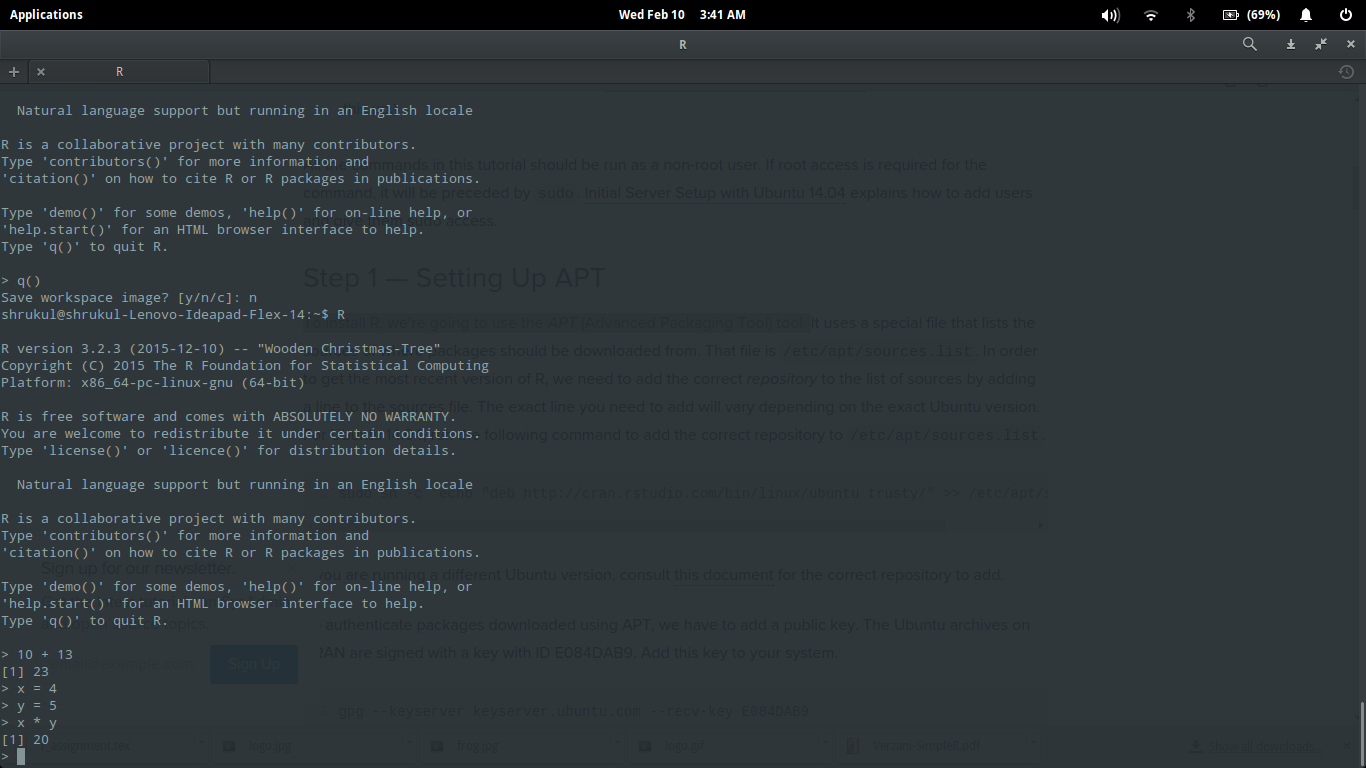
\includegraphics[scale=0.25]{r_window.png}
  \centering
  \caption{Running R in Linux}
  \label{fig:barchart1}
\end{figure}

\section{Basics of R}

\subsection{Input}

\subsubsection{Assignment}

The most straight forward way to store a list of numbers is through an assignment using the c command. (c stands for “combine.”) The idea is that a list of numbers is stored under a given name, and the name is used to refer to the data. A list is specified with the c command, and assignment is specified with the “<-” symbols. Another term used to describe the list of numbers is to call it a “vector.”

The numbers within the c command are separated by commas. As an example, we can create a new variable, called “bubba” which will contain the numbers 3, 5, 7, and 9: \newline

\begin{lstlisting}[frame=single]
> bubba <- c(3,5,7,9)
>
\end{lstlisting}

\clearpage

When you enter this command you should not see any output except a new command line. The command creates a list of numbers called “bubba.” To see what numbers is included in bubba type “bubba” and press the enter key: \newline

\begin{lstlisting}[frame=single]
> bubba
[1] 3 5 7 9
\end{lstlisting}

If you wish to work with one of the numbers you can get access to it using the variable and then square brackets indicating which number: \newline

\begin{lstlisting}[frame=single]
> bubba[2]
[1] 5
> bubba[1]
[1] 3
> bubba[0]
numeric(0)
> bubba[3]
[1] 7
> bubba[4]
[1] 9
\end{lstlisting}

\subsection{Basic Data Types}

We look at some of the ways that R can store and organize data. This is a basic introduction to a small subset of the different data types recognized by R and is not comprehensive in any sense.

\subsubsection{Numbers}

 The most basic way to store a number is to make an assignment of a single number: \newline
 
\begin{lstlisting}[frame=single]
> a <- 3
> a
[1] 3
\end{lstlisting}

To list all  the variables that you have defined in a particular session, use ls() \newline

\begin{lstlisting}[frame=single]
> ls()
[1] "a" "b"
\end{lstlisting}

\subsubsection{Strings}

 A string is specified by using quotes. Both single and double quotes will work: \newline

\begin{lstlisting}[frame=single]
> a <- "hello"
> a
[1] "hello"
> b <- c("hello","there")
> b
[1] "hello" "there"
> b[1]
[1] "hello"
\end{lstlisting}

\subsubsection{Logical}

Another important data type is the logical type. There are two predefined variables, TRUE and FALSE: \newline

\begin{lstlisting}[frame=single]
> a = TRUE
> typeof(a)
[1] "logical"
> b = FALSE
> typeof(b)
[1] "logical"
\end{lstlisting}

\clearpage

\section{Basic Operations and Numerical Descriptions}

We look at some of the basic operations that you can perform on lists of numbers. \newline

\subsection{Basic Operations}

Here we first define a vector which we will call “a” .First, the vector will contain the numbers 1, 2, 3, and 4. We then see how to add 5 to each of the numbers, subtract 10 from each of the numbers, multiply each number by 4, and divide each number by 5. \newline

\begin{lstlisting}[frame=single]
> a <- c(1,2,3,4)
> a
[1] 1 2 3 4
> a + 5
[1] 6 7 8 9
> a - 10
[1] -9 -8 -7 -6
> a*4
[1]  4  8 12 16
> a/5
[1] 0.2 0.4 0.6 0.8
\end{lstlisting}


We can save the results in another vector called b: \newline

\begin{lstlisting}[frame=single]
> b <- a - 10
> b
[1] -9 -8 -7 -6
\end{lstlisting}

\begin{itemize}
\item There are many inbuilt functions in R for statistical analysis. 
\item Such as mean(), median() and var() are some of the popular measures. 
\end{itemize}

So for our example:

\begin{lstlisting}[frame=single]
> vec = c(5,9,1,0)
> vec
[1] 5 9 1 0
> mean(vec)
[1] 3.75
> median(vec)
[1] 3
> var(vec)
[1] 16.91667
\end{lstlisting}

If you want to take the square root, find e raised to each number, the logarithm, etc., then the usual commands can be used: \newline

\begin{lstlisting}[frame=single]
> sqrt(a)
[1] 1.000000 1.414214 1.732051 2.000000
> exp(a)
[1]  2.718282  7.389056 20.085537 54.598150
> log(a)
[1] 0.0000000 0.6931472 1.0986123 1.3862944
> exp(log(a))
[1] 1 2 3 4
> c <- (a + sqrt(a))/(exp(2)+1)
> c
[1] 0.2384058 0.4069842 0.5640743 0.7152175
\end{lstlisting}

The operation is performed on an element by element basis.  \newline

\begin{lstlisting}[frame=single]
> a*b
[1]  -9 -16 -21 -24
> a/b
[1] -0.1111111 -0.2500000 -0.4285714 -0.6666667
> (a+3)/(sqrt(1-b)*2-1)
[1] 0.7512364 1.0000000 1.2884234 1.6311303
\end{lstlisting}

\clearpage

The summary command will print out the min, max, mean, median, and quantiles:\\

\begin{lstlisting}[frame=single]
> data = c(15,20,26,14,25,39,12)
> summary(data)
   Min. 1st Qu.  Median    Mean 3rd Qu.    Max. 
  12.00   14.50   20.00   21.57   25.50   39.00 
\end{lstlisting}

\section{Plotting Functions}

We look at some of the ways R can display information graphically. This is a basic introduction to some of the basic plotting commands. 

\subsection{Bar Charts}

A bar chart draws a bar with a a height proportional to the count in the table. The height could be given by the
frequency, or the proportion. The graph will look the same, but the scales may be different.

Sample bar chart is given:

\begin{lstlisting}[frame=single ]
> bar = c(5,2,1,6,3,9,7,8,3,2,6,3,5,3,1,7)
> barplot(table(bar))
\end{lstlisting} 

\clearpage
The Output of the above program is :\\

\begin{figure}[h!]
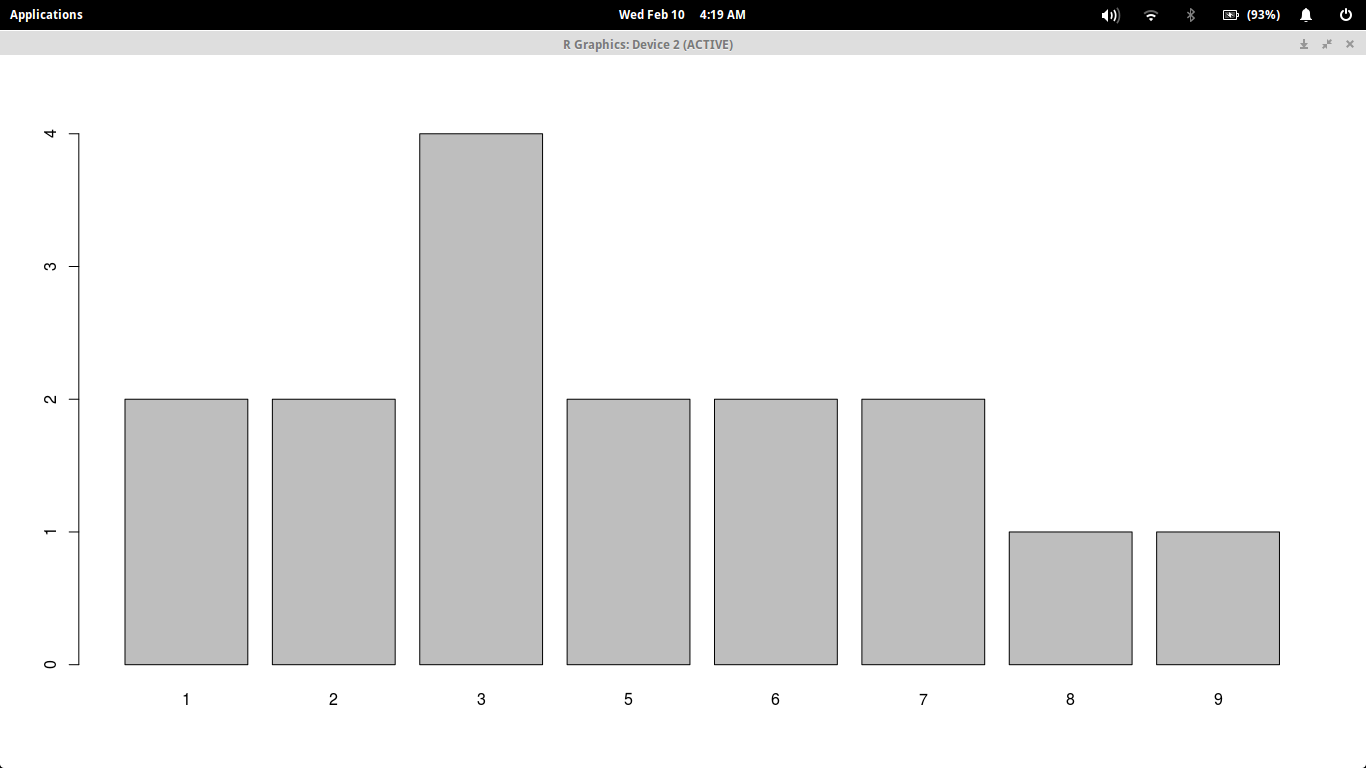
\includegraphics[scale=0.35]{bar_plot.png}
  \centering
  \caption{Bar chart}
  \label{fig:barchart1}
\end{figure}

\clearpage

\subsection{Simple Pie Chart}
We can also draw Pie Charts similarly using the pie() function as show below:\\

\begin{lstlisting}[frame=single]
> slices = c(1,2,1,4,1,5,4,1,2,5)
> lbls <- c("One", "Two", "Three", "Four", "Five", "Six", "Seven", "Eight", "Nine", "Ten")
> pie(slices, labels = lbls, main="Pie Chart of Countries")
\end{lstlisting} 

So we will get pie chart like this:\\

 
\begin{figure}[h!]
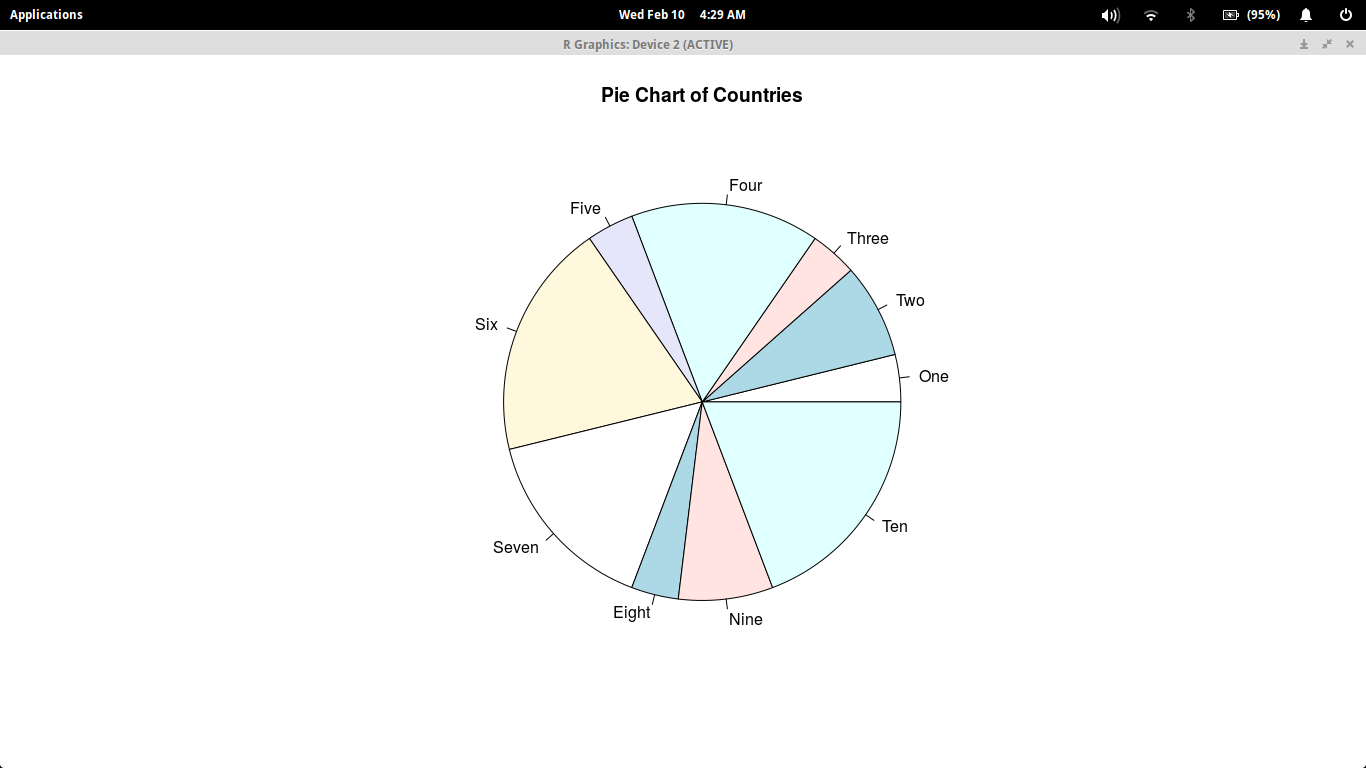
\includegraphics[scale=0.35]{pie_plot.png}
  \centering
  \caption{Pie chart}
  \label{fig:barchart1}
\end{figure}

\clearpage

\subsection{Strip Charts}

A strip chart is the most basic type of plot available. It plots the data in order along a line with each data point represented as a box.\\

To create a strip chart of this data use the stripchart command:\\

\begin{lstlisting}[frame=single]
> var = c(5,2,1,6,3,9,7,8,3,2,6,3,5,3,1,7)
> stripchart(var)
\end{lstlisting} 

So we will get Strip chart like this:\\

 
\begin{figure}[h!]
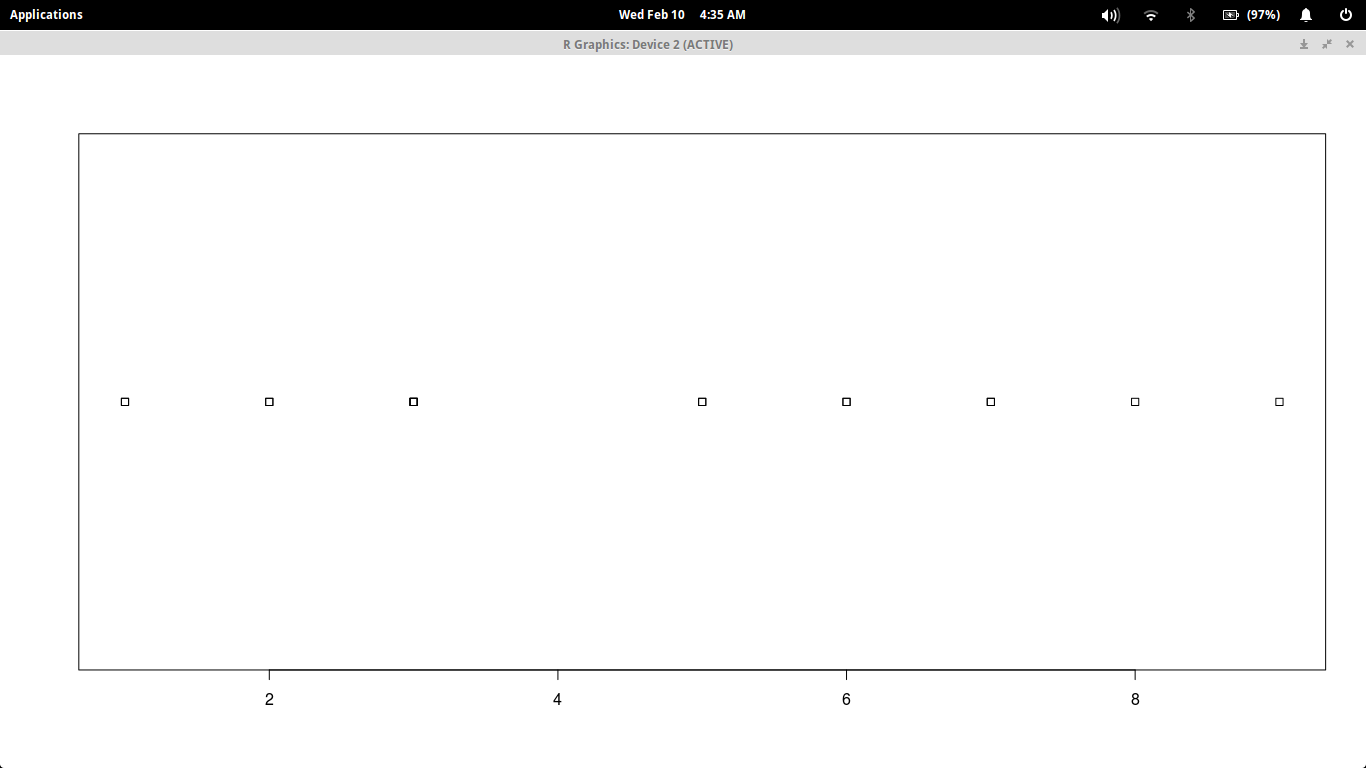
\includegraphics[scale=0.35]{strip_plot.png}
  \centering
  \caption{Strip chart}
  \label{fig:barchart1}
\end{figure}

\clearpage

\subsection{Histogram}

A histogram is very common plot. It plots the frequencies that data appears within certain ranges.
The histogram defines a sequence of breaks and then counts the number of observation in the bins formed by the breaks. \\ 
To create a Histogram of this data use the stripchart command:\\

\begin{lstlisting}[frame=single]
> var = c(5,2,1,6,3,9,7,8,3,2,6,3,5,3,1,7)
> hist(var)
\end{lstlisting} 

So we will get the Histogram like this:\\

 
\begin{figure}[h!]
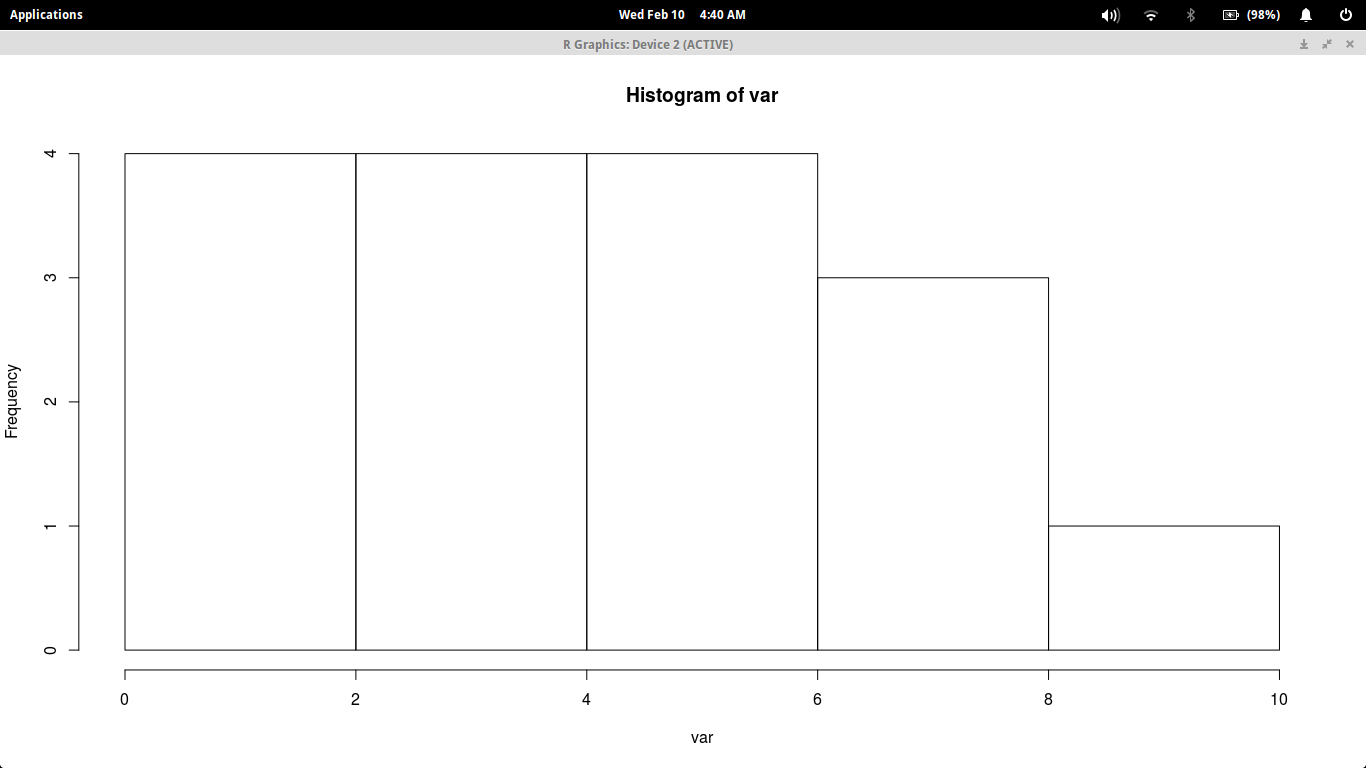
\includegraphics[scale=0.35]{hist_plot.png}
  \centering
  \caption{Histogram}
  \label{fig:barchart1}
\end{figure}

\section{Bivariate data}
Bivariate data is used to combine two variables and it is summarized using table. We can use bivariate data by creating two independent vectors and then combining them using table command.

\begin{lstlisting}[frame=single ]
> mobile = c("samsung","xiaomi","samsung","micromax","intex","yu","oneplus","samsung","lenovo","xiaomi","micromax",
"htc","oneplus","lenovo","samsung","micromax")
> value = c(1,2,5,2,1,5,2,1,5,2,1,3,2,5,1,2)
> table(mobile,value)
          value
mobile     1 2 3 5
  htc      0 0 1 0
  intex    1 0 0 0
  lenovo   0 0 0 2
  micromax 1 2 0 0
  oneplus  0 2 0 0
  samsung  3 0 0 1
  xiaomi   0 2 0 0
  yu       0 0 0 1
> barplot(table(mobile,value),col=c("purple","green2"),beside=TRUE)
\end{lstlisting}

If more than one measurement is made on each observation, multivariate analysis is applied.
With bivariate analysis, we are testing hypotheses of ”association” and causality. In its simplest form, association
simply refers to the extent to which it becomes easier to know/predict a value for the Dependent variable if we know
a case’s value on the independent variable. \\
A measure of association helps us to understand this relationship. These measures of association relate to how much
better this prediction becomes with knowledge of the IV or how well an independent variable relates to the dependent
variable. We have already discussed this in more abstract terms of ”correlation”. A measure of association often
ranges between 1 and 1.Where the sign of the integer represents the ”direction” of correlation (negative or positive
relationships) and the distance away from 0 represents the degree or extent of correlation the farther the number away
from 0, the higher or ”more perfect” the relationship is between the IV and DV.

\subsection{Linear regression}

One of the most frequent used techniques in statistics is linear regression where we investigate the potential relationship between a variable of interest (often called the response variable but there are many other names in use) and a set of one of more variables (known as the independent variables or some other term). Unsurprisingly there are flexible facilities in R for fitting a range of linear models from the simple case of a single variable to more complex relationships. \\

\subsection{For Nominal Variables}
Measure of association is Lambda. Literally, lambda is the extent to which guessing the values of the dependent vari-
able is improved by knowing which category the case falls in for the IV. The formula for Lambda is \\

lambda = (Reduction in Error from guessing to predicting based on IV)/ Number of Original Error \\

This gives you a ratio of how much improvement your prediction has by knowing values on the IV. Lambda ranges
from 0 to 1. (Remember, there is no order to nominal variables, therefore, you can not predict a ”direction” of
association). The higher the number, the stronger the relationship between the two variables.

\subsection{For ordinal variables}
The appropriate measures of association all attempt to measure how values of ordered variables relate for the sample of cases. For instance, how many times are high values associated with high values, how many times are they associated
with low values. They each use discordant and concordant pairs to create a value between 1 and 1. O indicates no
relationship between how the values for the cases pair up. The closer to 1 means the stronger the negative (inverse)
relationship, and the closer to 1 the more ”perfect” the positive relationship. There are several measures of association which measure ordinal variables’ relationships. Somer’s d, tau b, tau c, and gamma are the most usual ones. All are slight variations of the formula related in layman’s terms above. While Somer’s d, tau b, and tau c will all have very close to the same value, gamma usually will appear to have a slightly higher (stronger) relationship.

\subsection{For interval variables}
One statistic that is often used with interval data is the t-test. This statistics tests whether two subgroups of a sample have large enough difference between their means that the difference actually exists (is statistically significant).

\section{Conclusion}

The R programming language is an important tool for development in the numeric analysis and machine learning spaces. With machines becoming more important as data generators, the popularity of the language can only be expected to grow.\\

The main advantages of R language are:\\
\begin{itemize}
\item R is a powerful scripting language
\item Graphics and data visualization
\item Integration with document publishing
\item Access to powerful, cutting-edge analytics
\item No cost
\item R’s language has a powerful, easy to learn syntax with many built-in statistical functions.
\item Students can easily migrate to the commercially supported S-Plus program if commercial software is desired.
\item R is a computer programming language. For programmers it will feel more familiar than others and for new
computer users, the next leap to programming will not be so large.
\end{itemize}

\end{document}